\documentclass[11pt,a4paper]{article}
\usepackage[a4paper,margin=2cm]{geometry}
\usepackage[T1]{fontenc}
\usepackage{lmodern,microtype,amsmath,graphicx,booktabs,array,xurl}
\usepackage[numbers,sort&compress]{natbib}
\usepackage[hidelinks]{hyperref}
\usepackage{caption}
\captionsetup{font=small,labelfont=bf}
\setlength{\parindent}{1.3em}
\setlength{\parskip}{2pt}
\setlength{\bibsep}{1pt}
\setlength{\emergencystretch}{3em}
% Auto-generated by scripts/05_figures_tables.py from results/*.json. Do not edit.
\newcommand{\AUCciCART}{[0.739, 0.780]}
\newcommand{\AUCciLR}{[0.773, 0.812]}
\newcommand{\AUCciXGB}{[0.777, 0.815]}
\newcommand{\AgreeCARTXGB}{89.7\%}
\newcommand{\AgreeLRCART}{88.3\%}
\newcommand{\AgreeLRXGB}{94.2\%}
\newcommand{\AllNineBadRate}{54.9\%}
\newcommand{\BadRateMDENever}{39.8\%}
\newcommand{\BadRateMDEOneTwenty}{62.4\%}
\newcommand{\BadRatePop}{52.0\%}
\newcommand{\BgBaseSDFiftyXGB}{0.139}
\newcommand{\BgBaseSDTwoXGB}{0.088}
\newcommand{\BrierciCART}{[0.1912, 0.2097]}
\newcommand{\BrierciLR}{[0.1767, 0.1942]}
\newcommand{\BrierciXGB}{[0.1752, 0.1929]}
\newcommand{\CARTccp}{0.0005}
\newcommand{\CARTdepth}{5}
\newcommand{\CARTleaves}{18}
\newcommand{\CARTleavesMax}{19}
\newcommand{\CARTleavesMin}{16}
\newcommand{\CARTminleaf}{200}
\newcommand{\CARTpath}{4.4}
\newcommand{\CARTrootTop}{ExternalRiskEstimate}
\newcommand{\CARTrootTopN}{30}
\newcommand{\CARTvars}{6}
\newcommand{\CITLCART}{+0.006}
\newcommand{\CITLLR}{+0.005}
\newcommand{\CITLXGB}{+0.006}
\newcommand{\CVAUCCART}{0.781}
\newcommand{\CVAUCCARTdepthTwo}{0.757}
\newcommand{\CVAUCLR}{0.806}
\newcommand{\CVAUCXGB}{0.809}
\newcommand{\CVBrierCART}{0.1896}
\newcommand{\CVBrierLR}{0.1791}
\newcommand{\CVBrierXGB}{0.1778}
\newcommand{\CalSlopeCART}{0.83}
\newcommand{\CalSlopeLR}{0.95}
\newcommand{\CalSlopeXGB}{0.96}
\newcommand{\CaseDCART}{0.22}
\newcommand{\CaseDLR}{0.65}
\newcommand{\CaseDLeaf}{581}
\newcommand{\CaseDXGB}{0.71}
\newcommand{\CaseSAvgMInFile}{383}
\newcommand{\CaseSCART}{0.79}
\newcommand{\CaseSLR}{0.47}
\newcommand{\CaseSLRAvg}{$-$2.34}
\newcommand{\CaseSLeaf}{342}
\newcommand{\CaseSMissingSplits}{4}
\newcommand{\CaseSNSpecial}{9}
\newcommand{\CaseSPathLen}{5}
\newcommand{\CaseSXGB}{0.74}
\newcommand{\CaseSXGBAvg}{$-$0.32}
\newcommand{\CaseTCART}{0.49}
\newcommand{\CaseTLR}{0.50}
\newcommand{\CaseTLeaf}{307}
\newcommand{\CaseTXGB}{0.51}
\newcommand{\ConflictBgFiftyLR}{11.3\%}
\newcommand{\ConflictBgFiftyXGB}{4.6\%}
\newcommand{\ConflictBgTwoXGB}{1.8\%}
\newcommand{\ConflictRtLR}{5.4\%}
\newcommand{\ConflictRtXGB}{9.9\%}
\newcommand{\ConflictSdXGB}{4.1\%}
\newcommand{\FlipRtCART}{22.4\%}
\newcommand{\FlipRtLR}{5.0\%}
\newcommand{\FlipRtXGB}{8.3\%}
\newcommand{\FlipSdXGB}{5.6\%}
\newcommand{\GtTenLRXGB}{12.4\%}
\newcommand{\LRC}{0.048}
\newcommand{\LRalways}{20}
\newcommand{\LRnnz}{30}
\newcommand{\LRnnzMax}{35}
\newcommand{\LRnnzMin}{26}
\newcommand{\LRsignflip}{0}
\newcommand{\LRsometimes}{23}
\newcommand{\LRvars}{19}
\newcommand{\MeanAbsLRXGB}{0.050}
\newcommand{\NAllNine}{588}
\newcommand{\NCols}{46}
\newcommand{\NDev}{7,896}
\newcommand{\NEval}{303}
\newcommand{\NPartialNine}{10}
\newcommand{\NPop}{9,871}
\newcommand{\NRaw}{10,459}
\newcommand{\NRepeats}{10}
\newcommand{\NRuns}{30}
\newcommand{\NTest}{1,975}
\newcommand{\NegInqEightOR}{30}
\newcommand{\NegInqSevenOR}{0}
\newcommand{\NegMDEOneTwenty}{30}
\newcommand{\NegMDTwelveOneTwenty}{27}
\newcommand{\ORInqEightOR}{0.39}
\newcommand{\ORInqSevenOR}{1.23}
\newcommand{\ORMDEOneTwenty}{0.85}
\newcommand{\ORMDTwelveOneTwenty}{0.78}
\newcommand{\PathJacRtCART}{0.69}
\newcommand{\PredSDRtCART}{0.055}
\newcommand{\PredSDRtLR}{0.009}
\newcommand{\PredSDRtXGB}{0.017}
\newcommand{\PredSDSdXGB}{0.010}
\newcommand{\PredSDninetyRtCART}{0.085}
\newcommand{\PredSDninetyRtLR}{0.013}
\newcommand{\PredSDninetyRtXGB}{0.025}
\newcommand{\PredSDninetySdXGB}{0.015}
\newcommand{\RelLBgFiftyLR}{0.20}
\newcommand{\RelLBgFiftyXGB}{0.18}
\newcommand{\RelLBgTwoLR}{0.11}
\newcommand{\RelLBgTwoXGB}{0.10}
\newcommand{\RelLRtLR}{0.13}
\newcommand{\RelLRtXGB}{0.20}
\newcommand{\RelLSdXGB}{0.13}
\newcommand{\RepAUCCART}{0.773}
\newcommand{\RepAUCLR}{0.807}
\newcommand{\RepAUCXGB}{0.808}
\newcommand{\RepAUCsdCART}{0.014}
\newcommand{\RepAUCsdLR}{0.011}
\newcommand{\RepAUCsdXGB}{0.010}
\newcommand{\RepAucDiffLRCART}{0.0337}
\newcommand{\RepAucDiffMaxLRCART}{0.0454}
\newcommand{\RepAucDiffMaxXGBCART}{0.0474}
\newcommand{\RepAucDiffMaxXGBLR}{0.0066}
\newcommand{\RepAucDiffMinLRCART}{0.0284}
\newcommand{\RepAucDiffMinXGBCART}{0.0268}
\newcommand{\RepAucDiffMinXGBLR}{$-$0.0032}
\newcommand{\RepAucDiffPosLRCART}{10}
\newcommand{\RepAucDiffPosXGBCART}{10}
\newcommand{\RepAucDiffPosXGBLR}{6}
\newcommand{\RepAucDiffXGBCART}{0.0345}
\newcommand{\RepAucDiffXGBLR}{0.0008}
\newcommand{\RepBrierCART}{0.1924}
\newcommand{\RepBrierDiffLRCART}{$-$0.0135}
\newcommand{\RepBrierDiffMaxLRCART}{$-$0.0116}
\newcommand{\RepBrierDiffMaxXGBCART}{$-$0.0110}
\newcommand{\RepBrierDiffMaxXGBLR}{0.0010}
\newcommand{\RepBrierDiffMinLRCART}{$-$0.0169}
\newcommand{\RepBrierDiffMinXGBCART}{$-$0.0179}
\newcommand{\RepBrierDiffMinXGBLR}{$-$0.0032}
\newcommand{\RepBrierDiffPosLRCART}{0}
\newcommand{\RepBrierDiffPosXGBCART}{0}
\newcommand{\RepBrierDiffPosXGBLR}{3}
\newcommand{\RepBrierDiffXGBCART}{$-$0.0141}
\newcommand{\RepBrierDiffXGBLR}{$-$0.0005}
\newcommand{\RepBrierLR}{0.1789}
\newcommand{\RepBrierXGB}{0.1784}
\newcommand{\SelInqEightOR}{30}
\newcommand{\SelInqSevenOR}{30}
\newcommand{\SelMDEOneTwenty}{30}
\newcommand{\SelMDTwelveOneTwenty}{27}
\newcommand{\SignBgFiftyLR}{0.83}
\newcommand{\SignBgFiftyXGB}{0.86}
\newcommand{\SignBgTwoLR}{0.93}
\newcommand{\SignBgTwoXGB}{0.91}
\newcommand{\SignRtLR}{0.74}
\newcommand{\SignRtXGB}{0.76}
\newcommand{\SignSdXGB}{0.80}
\newcommand{\SwapBaseAll}{+0.14}
\newcommand{\SwapBaseBad}{+0.77}
\newcommand{\SwapBaseGood}{$-$0.73}
\newcommand{\SwapTAll}{$-$0.12}
\newcommand{\SwapTBad}{$-$0.75}
\newcommand{\SwapTGood}{+0.75}
\newcommand{\TestAUCCART}{0.758}
\newcommand{\TestAUCLR}{0.792}
\newcommand{\TestAUCXGB}{0.796}
\newcommand{\TestBrierCART}{0.2009}
\newcommand{\TestBrierLR}{0.1856}
\newcommand{\TestBrierXGB}{0.1843}
\newcommand{\TestLLCART}{0.589}
\newcommand{\TestLLLR}{0.554}
\newcommand{\TestLLXGB}{0.549}
\newcommand{\TopFiveBgFiftyLR}{0.87}
\newcommand{\TopFiveBgFiftyXGB}{0.91}
\newcommand{\TopFiveBgTwoLR}{0.93}
\newcommand{\TopFiveBgTwoXGB}{0.96}
\newcommand{\TopFiveRtLR}{0.90}
\newcommand{\TopFiveRtXGB}{0.91}
\newcommand{\TopFiveSdXGB}{0.94}
\newcommand{\TopThreeBgFiftyLR}{0.88}
\newcommand{\TopThreeBgFiftyXGB}{0.86}
\newcommand{\TopThreeBgTwoLR}{0.93}
\newcommand{\TopThreeBgTwoXGB}{0.92}
\newcommand{\TopThreeRtLR}{0.92}
\newcommand{\TopThreeRtXGB}{0.88}
\newcommand{\TopThreeSdXGB}{0.93}
\newcommand{\XGBdepth}{3}
\newcommand{\XGBeta}{0.022}
\newcommand{\XGBleaves}{2,255}
\newcommand{\XGBntrees}{290}
\newcommand{\XGBtrees}{290}
\newcommand{\XGBvars}{23}
\newcommand{\dAUCCARTXGB}{$-$0.037}
\newcommand{\dAUCLRCART}{0.034}
\newcommand{\dAUCLRXGB}{$-$0.003}
\newcommand{\dAUCciCARTXGB}{[$-$0.046, $-$0.028]}
\newcommand{\dAUCciLRCART}{[0.023, 0.045]}
\newcommand{\dAUCciLRXGB}{[$-$0.009, 0.002]}
\newcommand{\dBrierCARTXGB}{0.0166}
\newcommand{\dBrierLRCART}{$-$0.0153}
\newcommand{\dBrierLRXGB}{0.0013}
\newcommand{\dBrierciCARTXGB}{[0.0126, 0.0205]}
\newcommand{\dBrierciLRCART}{[$-$0.0201, $-$0.0103]}
\newcommand{\dBrierciLRXGB}{[$-$0.0014, 0.0040]}

% Auto-generated from the completed exploratory ablation. Do not edit.
\newcommand{\GapFullXGBLR}{+0.003}
\newcommand{\GapNoScoreXGBLR}{+0.003}
\newcommand{\NNoScoreCols}{44}
\newcommand{\NNoScoreVars}{22}
\newcommand{\NoScoreAUCCART}{0.754}
\newcommand{\NoScoreAUCLR}{0.791}
\newcommand{\NoScoreAUCXGB}{0.794}
\newcommand{\NoScoreBrierCART}{0.2001}
\newcommand{\NoScoreBrierLR}{0.1861}
\newcommand{\NoScoreBrierXGB}{0.1850}
\newcommand{\NoScoreChangeTenCART}{46.8\%}
\newcommand{\NoScoreChangeTenLR}{1.2\%}
\newcommand{\NoScoreChangeTenXGB}{5.8\%}
\newcommand{\NoScoreLRCoef}{33}
\newcommand{\NoScoreLRVars}{20}
\newcommand{\NoScoreLabelChangeCART}{16.5\%}
\newcommand{\NoScoreLabelChangeLR}{3.0\%}
\newcommand{\NoScoreLabelChangeXGB}{4.9\%}
\newcommand{\NoScoreMeanChangeCART}{0.121}
\newcommand{\NoScoreMeanChangeLR}{0.026}
\newcommand{\NoScoreMeanChangeXGB}{0.036}
\newcommand{\RepScoreAUCMeanCART}{+0.0083}
\newcommand{\RepScoreAUCMeanLR}{+0.0011}
\newcommand{\RepScoreAUCMeanXGB}{+0.0006}
\newcommand{\RepScoreAUCPosCART}{8}
\newcommand{\RepScoreAUCPosLR}{9}
\newcommand{\RepScoreAUCPosXGB}{7}
\newcommand{\ScoreDeltaAUCCART}{+0.004}
\newcommand{\ScoreDeltaAUCLR}{+0.001}
\newcommand{\ScoreDeltaAUCXGB}{+0.001}
\newcommand{\ScoreDeltaAUCciCART}{[$-$0.011, 0.019]}
\newcommand{\ScoreDeltaAUCciLR}{[$-$0.002, 0.005]}
\newcommand{\ScoreDeltaAUCciXGB}{[$-$0.003, 0.006]}
\newcommand{\ScoreDeltaBrierCART}{+0.0008}
\newcommand{\ScoreDeltaBrierLR}{$-$0.0005}
\newcommand{\ScoreDeltaBrierXGB}{$-$0.0006}
\newcommand{\ScoreDeltaBrierciCART}{[$-$0.0058, 0.0072]}
\newcommand{\ScoreDeltaBrierciLR}{[$-$0.0020, 0.0010]}
\newcommand{\ScoreDeltaBrierciXGB}{[$-$0.0027, 0.0013]}

\newcommand{\var}[1]{{\small\nolinkurl{#1}}}
\title{\vspace{-1.2cm}Interpretable models and explained black boxes:\\a credit-risk case study}
\author{Zijing LIU, Jiahao WANG, Ziyue WANG, Yirong YANG, Qianwei YU}
\date{November 2026}
\begin{document}
\maketitle
\vspace{-0.7cm}
\begin{abstract}
We compare L1 logistic regression, depth-limited CART and XGBoost on FICO HELOC credit-risk data, separating prediction quality, inspectability and validation. Logistic regression and XGBoost have close observed test AUCs (\TestAUCLR{} and \TestAUCXGB{}), while CART performs worse. An exploratory removal of an undocumented upstream score preserves that proximity, but substantially changes many individual CART probabilities. Refitting and reference-sample analyses reveal different sources of variation in explanations. These results support considering inspectable alternatives and auditing their behaviour, without establishing model equivalence, causal explanations or deployment validity.
\end{abstract}

\section{Question and conceptual framework}
We ask how much predictive performance differs between selected interpretable models and XGBoost, what their structures and explanations reveal, and which validation gaps remain. This is a controlled empirical comparison and model audit, not a new algorithm.

Rudin argues against assuming an unavoidable accuracy--interpretability trade-off in high-stakes structured prediction and advocates inherently interpretable alternatives \cite{rudin2019stop}. Murdoch et al.'s predictive--descriptive--relevant (PDR) framework distinguishes predictive quality, faithful description of learned relationships and usefulness to a particular audience \cite{murdoch2019definitions}. Ghassemi et al. emphasise that local explanations cannot certify individual decisions and that validation must carry that burden; their medical evidence is not direct credit evidence \cite{ghassemi2021false}. Goodman and Flaxman motivate explanation and non-discrimination requirements \cite{goodman2017eu}; we do not assess current legal compliance.

Here, logistic regression and CART expose a fitted equation or decision path; XGBoost is computationally complex and is analysed with post-hoc TreeSHAP. The terminology is operational, not universal. Nonlinear interpretable alternatives also exist \cite{chen2022holistic}, but are outside our implemented model classes. Inspectable computation is not necessarily easy for an applicant to understand.

\section{Data and experimental protocol}
HELOC contains \NRaw{} records and 23 bureau predictors. We encode Bad as 1. FICO's description through IBM AIX360 defines Bad as 90+ days past due at least once within 24 months of account opening \cite{aix360heloc}; the available dictionary says 12--36 months. Official originals were unavailable, so we disclose this discrepancy and use a raw secondary copy verified by SHA-256. The target is repayment performance, not approval; sampling and acceptance selection cannot be verified.

We exclude \NAllNine{} records with all predictors equal to $-9$, restricting inference to \NPop{} records with bureau information (\BadRatePop{} Bad). Special codes $-7$, $-8$ and $-9$ denote different states, not ordinary negative values: numeric entries become missing with explicit indicators. Two coded delinquency fields are one-hot encoded, yielding \NCols{} shared inputs. An exact duplicate pair is kept within one split. Logistic imputation and standardisation are fitted only on training portions; trees handle missing inputs natively.

A group-aware stratified split reserves \NTest{} test records; \NDev{} development records share five CV folds. Mean CV Brier selects among 20 logistic penalties, 80 CART configurations (depth 2--5) and 60 XGBoost configurations. XGBoost stops on a training-fold internal slice; the final tree count is the median selected stopping point. Ten additional 75/25 development splits repeat selection with three inner folds. They overlap and are reported descriptively. Test paired percentile bootstrap intervals use 2,000 resamples and condition on fitted models. AUC measures ranking; Brier and log-loss measure overall probability quality, not calibration alone. Reliability and recalibration slopes are diagnostic, not test-set recalibration.

\section{Prediction, explanations and sensitivity}
Table~\ref{tab:results} reports final-test results. The logistic-minus-XGBoost AUC difference is \dAUCLRXGB{} (95\% interval \dAUCciLRXGB); its Brier difference is \dBrierLRXGB{} \dBrierciLRXGB. Inclusion of zero does not establish equivalence. Across development splits, their mean AUC difference (XGBoost minus logistic) is \RepAucDiffXGBLR{}. Restricted CART performs worse; this does not generalise to all interpretable models.

\begin{table}[htbp]
\centering\small
\caption{Test performance with all inputs and after score removal. No-score models are independently retuned; these comparisons are exploratory.}
\label{tab:results}
\begin{tabular}{@{}llrrrr@{}}
\toprule
Model & Inputs & AUC & Brier & Log-loss & Cal. slope \\
\midrule
L1 logistic & Full & 0.792 & 0.1856 & 0.554 & 0.95 \\
L1 logistic & No score & 0.791 & 0.1861 & 0.556 & 0.93 \\
CART & Full & 0.758 & 0.2009 & 0.589 & 0.83 \\
CART & No score & 0.754 & 0.2001 & 0.588 & 0.86 \\
XGBoost & Full & 0.796 & 0.1843 & 0.549 & 0.96 \\
XGBoost & No score & 0.794 & 0.1850 & 0.551 & 0.91 \\
\bottomrule
\end{tabular}

\end{table}

Aggregate proximity hides individual differences: \GtTenLRXGB{} of test customers receive logistic and XGBoost probabilities more than 0.10 apart. The full logistic model has \LRnnz{} non-zero coefficients on \LRvars{} original variables; CART has depth \CARTdepth{} and \CARTleaves{} leaves; XGBoost has \XGBtrees{} trees. These describe structure, not a common human-understanding score.

For the same rule-selected cases we examine logistic contributions, complete CART paths with leaf support, and TreeSHAP \cite{lundberg2020local}. Contributions are on the log-odds scale relative to 200 development records. TreeSHAP is deterministic for fixed inputs/settings and passes output reconstruction; neither property proves causal meaning or complete descriptive accuracy. Column contributions are summed to original variables, not recomputed as group Shapley values. Independent perturbations may create invalid joint encoded states. Readable paths also expose questionable missing-value routings. A stable negative coefficient for a severe-delinquency category motivates domain review; correlated conditional effects mean it is not automatically an error.

Figure~\ref{fig:cases} illustrates why inspecting mechanism adds information beyond an AUC comparison. For the maximum-disagreement case, logistic regression, XGBoost and CART assign \CaseDLR{}, \CaseDXGB{} and \CaseDCART{} risk. The complete CART path does not inspect satisfactory-trade count, a leading factor for the other models. In the special-code case, a missing score follows the low-score branch, ``no inquiries'' follows the recent-inquiry branch, and no usable revolving trades follows the high-burden branch. These are learned missing-input routings, not imputations of actual customer characteristics. They can be reproduced and questioned without establishing which prediction is correct for that individual.

\begin{figure}[htbp]
\centering
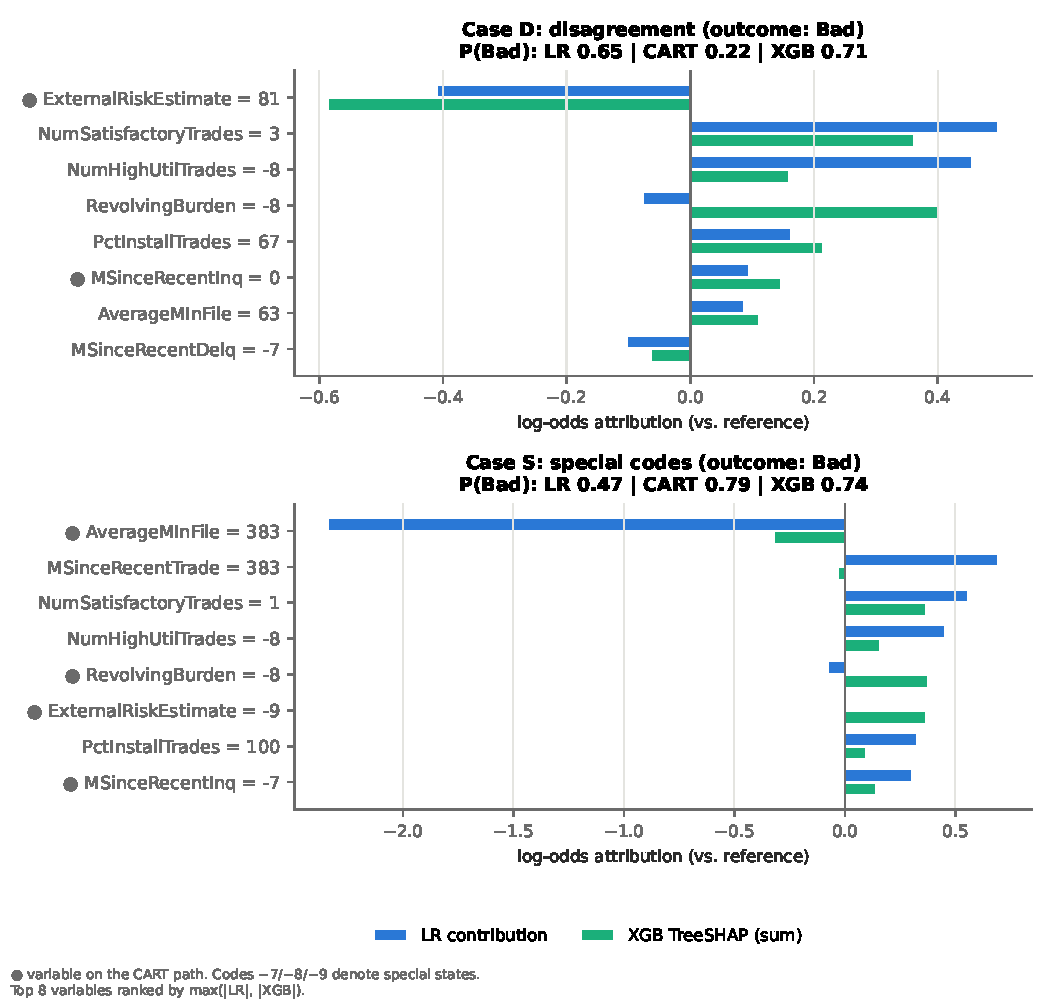
\includegraphics[width=0.95\textwidth]{../results/figures/fig2_cases.pdf}
\caption{Two rule-selected cases. Bars compare grouped logistic and XGBoost log-odds contributions against the same reference. The complete CART paths and all five cases accompany the research notes. Illustrations are not representative population evidence.}
\label{fig:cases}
\end{figure}

Thirty fixed-hyperparameter refits vary both a 90\% development subsample and seed, measuring combined variation; a separate XGBoost arm varies only seed. In \NEval{} fixed cases, mean prediction standard deviations are \PredSDRtLR{}, \PredSDRtCART{} and \PredSDRtXGB{}. No formal Rashomon set is constructed. With models fixed, 30 background redraws from the same population examine reference estimation separately (Fig.~\ref{fig:stability}). XGBoost top-3 variable overlap rises from \TopThreeBgFiftyXGB{} at 50 background records to \TopThreeBgTwoXGB{} at 200. Logistic contributions also depend on reference samples, although its equation does not. Changing the reference population changes the question rather than merely adding algorithmic noise.

\begin{figure}[htbp]
\centering
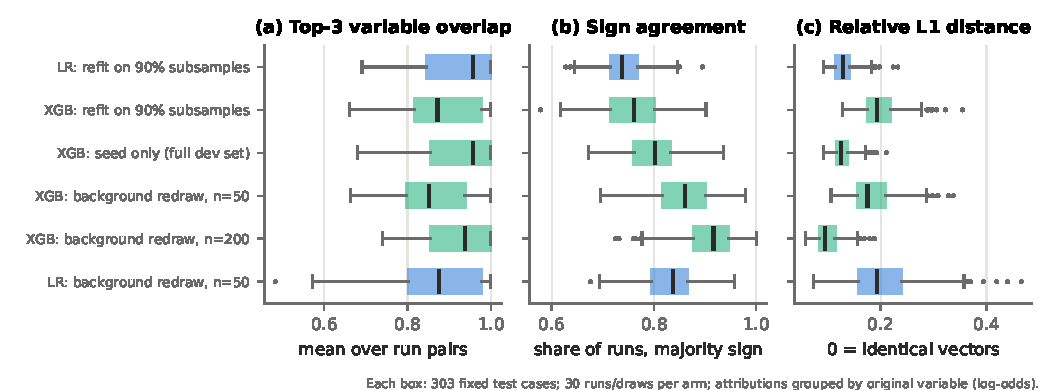
\includegraphics[width=\textwidth]{../results/figures/fig3_stability.pdf}
\caption{Grouped attribution stability. Refits change data and seed together; seed-only and background-redraw arms isolate other settings. Boxplots describe cases, not confidence that an explanation is correct.}
\label{fig:stability}
\end{figure}

\section{Exploratory upstream-score ablation}
All full-input models inherit \var{ExternalRiskEstimate}, whose construction is undocumented. We therefore remove the score and its derived indicator, keep all customer/split memberships, and retune all three families on the same grids. There are \NNoScoreVars{} remaining variables and \NNoScoreCols{} encoded columns. The analysis was designed after inspecting the main results and is exploratory.

The XGBoost-minus-logistic AUC gap is \GapFullXGBLR{} with the score and \GapNoScoreXGBLR{} without it. Their observed proximity therefore does not disappear on removal. Full-minus-no-score AUC intervals for logistic regression, CART and XGBoost are \ScoreDeltaAUCciLR{}, \ScoreDeltaAUCciCART{} and \ScoreDeltaAUCciXGB{}, respectively. These do not establish zero incremental value. In ten paired development splits, keeping the score gives higher AUC in \RepScoreAUCPosLR{} logistic, \RepScoreAUCPosCART{} CART and \RepScoreAUCPosXGB{} XGBoost comparisons. Remaining features may substitute for the score.

Individual probabilities change by more than 0.10 for \NoScoreChangeTenLR{}, \NoScoreChangeTenCART{} and \NoScoreChangeTenXGB{} of test customers (Fig.~\ref{fig:individual}). CART's small aggregate change thus coexists with substantial reassignment of risk. This compares independently retuned models, not a frozen-model intervention or a causal effect on customers. The 0.5 threshold is descriptive, not an optimal lending policy.

\begin{figure}[htbp]
\centering
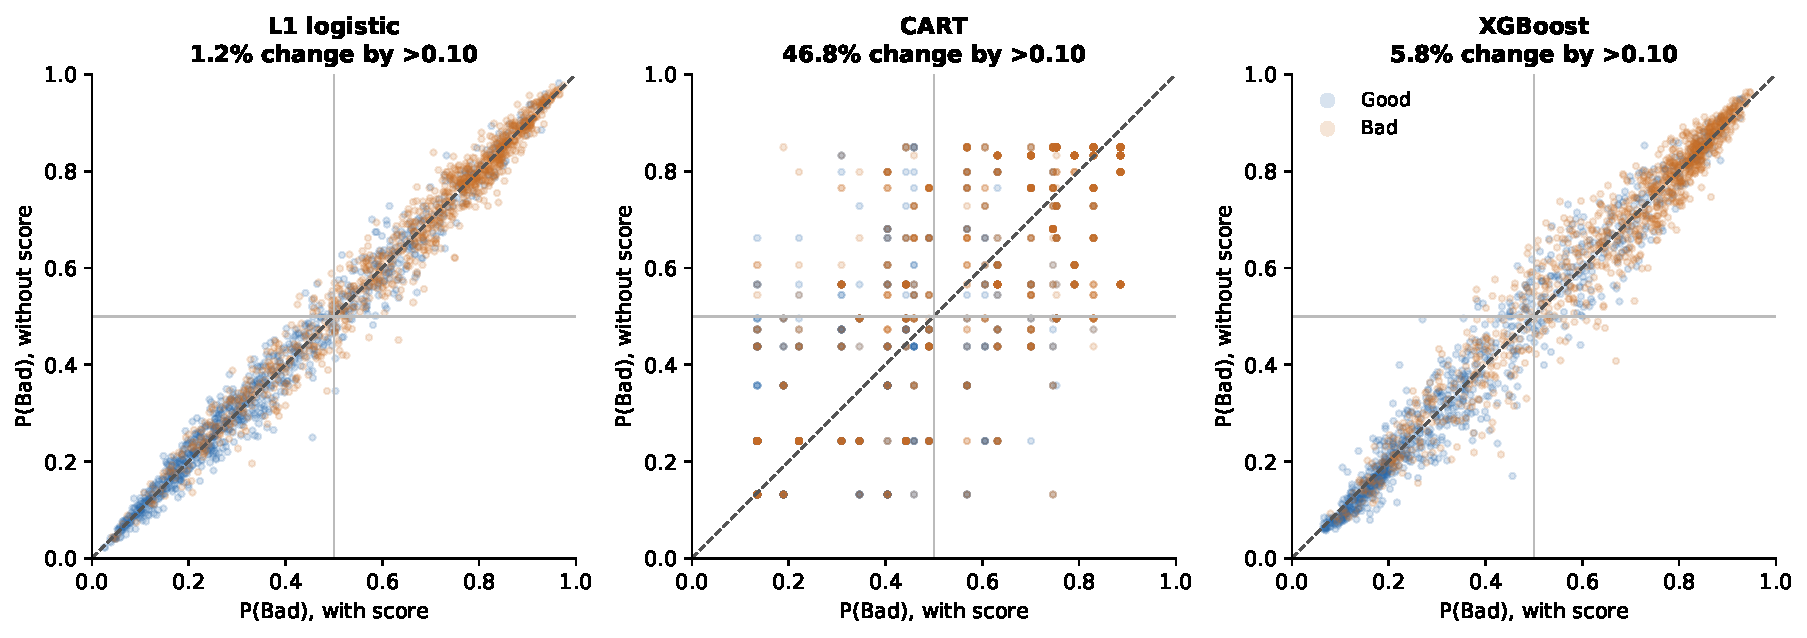
\includegraphics[width=\textwidth]{../results/figures/fig5_ablation_individual.pdf}
\caption{Same customers before and after score removal/refitting. The diagonal indicates unchanged probabilities. Colours are observed outcomes, not protected groups.}
\label{fig:individual}
\end{figure}

\section{Discussion, limitations and conclusion}
For PDR, predictive evidence supports considering logistic regression as an alternative in this task. Equations, paths and attributions provide inspectable information, but additivity and stability are not sufficient tests of descriptive quality. Audience relevance remains untested: developers, applicants and auditors need different information, and no user study was conducted. This supports Rudin's call to attempt interpretable alternatives while retaining Ghassemi et al.'s insistence on validation. Our reusable contribution is the comparison-and-audit workflow and its evidence, not an automatic deployment rule.

One historical dataset of uncertain sampling, secondary source material, limited model families and moderate tuning budgets restrict generalisation. No protected attributes are available, so fairness cannot be established. There is no temporal, institutional or prospective external validation, nor a decision-cost analysis. Similar average performance does not imply similar individual predictions, formal equivalence or deployment suitability. The score-removal extension strengthens one case-specific comparison without resolving all upstream opacity or the wider debate.

\noindent\textbf{Code availability.} Source, locked dependencies, saved results and reproduction instructions accompany the submission in \texttt{02\_Code/}; see \texttt{README.md} and \texttt{run\_all.sh}. Full methods, additional figures and editable sources are included in the research materials.

{\small\bibliographystyle{unsrtnat}\bibliography{refs}}
\end{document}
